\documentclass[border=6pt]{standalone}
% Shared preamble for web figures.  Each figure is a standalone .tex that
% \input's this file; scripts/make-figures.sh turns it into an SVG.
% Handouts pull the same file with \fig{Unit_X/<name>}.
\usepackage[T1]{fontenc}
\usepackage{helvet}
\renewcommand{\familydefault}{\sfdefault}
\renewcommand{\ttdefault}{pcr}  % Courier: a real Type 1 typewriter font
\usepackage{amsmath}
\usepackage{tikz}
\usetikzlibrary{arrows.meta,positioning,calc,shapes.symbols,shapes.geometric}

% Who makes the rules is the point of most diagrams in this book, so the
% colors mean the same thing everywhere: blue is a person, orange is the
% computer, green is an answer, pink is the human brain.
\definecolor{person}{HTML}{2C6FAE}
\definecolor{machine}{HTML}{D35400}
\definecolor{result}{HTML}{1E8449}
\definecolor{brainpink}{HTML}{C2185B}
\definecolor{ink}{HTML}{2C3E50}

\tikzset{
  doodle/.style={line width=1.5pt, line cap=round, line join=round, draw=ink},
  box/.style={draw, rounded corners=5pt, line width=1.1pt, align=center,
              inner sep=7pt, minimum height=1.0cm, font=\small},
  personbox/.style={box, draw=person, fill=person!10},
  machinebox/.style={box, draw=machine, fill=machine!10},
  resultbox/.style={box, draw=result, fill=result!10},
  plainbox/.style={box, draw=ink!70, fill=ink!4},
  flow/.style={-{Stealth[length=8pt]}, line width=1.4pt, draw=ink},
}

% A person (blue) and a robot head (orange) as small icons.
% \personicon{x}{y}{scale}   \roboticon{x}{y}{scale}
\newcommand{\personicon}[3]{%
  \begin{scope}[shift={(#1,#2)}, scale=#3]
    \fill[person] (0,0.62) circle (0.28);
    \fill[person, rounded corners=6pt] (-0.42,-0.55) rectangle (0.42,0.28);
  \end{scope}}
\newcommand{\roboticon}[3]{%
  \begin{scope}[shift={(#1,#2)}, scale=#3]
    \draw[machine, line width=1.2pt] (0,0.5) -- (0,0.72);
    \fill[machine] (0,0.78) circle (0.08);
    \draw[machine, line width=1.4pt, fill=machine!12, rounded corners=4pt] (-0.5,-0.45) rectangle (0.5,0.5);
    \fill[ink] (-0.2,0.12) circle (0.08);
    \fill[ink] (0.2,0.12) circle (0.08);
    \draw[ink, line width=1pt] (-0.22,-0.22) -- (0.22,-0.22);
  \end{scope}}

\begin{document}
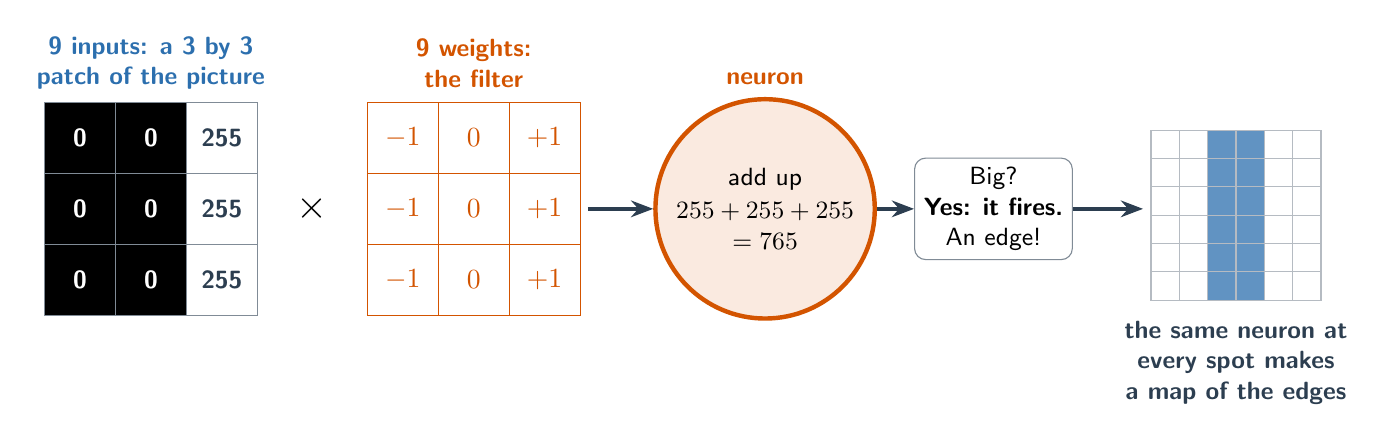
\begin{tikzpicture}[
  px/.style={draw=ink!60, minimum size=0.9cm, inner sep=0pt, font=\small\bfseries},
  wt/.style={draw=machine, fill=white, minimum size=0.9cm, inner sep=0pt, font=\normalsize\bfseries, text=machine},
]
% A filter is a neuron with 9 inputs: a 3 by 3 patch of the picture.
% Patch at an edge: dark (0) on the left, light (255) on the right.
\foreach \r in {0,1,2} {
  \node[px, fill=black, text=white] at (0,-\r*0.9) {0};
  \node[px, fill=black, text=white] at (0.9,-\r*0.9) {0};
  \node[px, fill=white, text=ink] at (1.8,-\r*0.9) {255};
}
\node[font=\small\bfseries, text=person, align=center] at (0.9,0.95) {9 inputs: a 3 by 3\\patch of the picture};
\node[font=\Large] at (2.95,-0.9) {$\times$};
\foreach \r in {0,1,2} {
  \node[wt] at (4.1,-\r*0.9) {$-1$};
  \node[wt] at (5.0,-\r*0.9) {$0$};
  \node[wt] at (5.9,-\r*0.9) {$+1$};
}
\node[font=\small\bfseries, text=machine, align=center] at (5.0,0.95) {9 weights:\\the filter};
\node[draw=machine, fill=machine!12, circle, line width=1.6pt, minimum size=2.3cm, align=center, font=\small] (n) at (8.7,-0.9)
  {add up\\[1pt]$255 + 255 + 255$\\$= 765$};
\draw[flow] (6.45,-0.9) -- (n);
\node[font=\small\bfseries, text=machine] at (8.7,0.75) {neuron};
\node[draw=ink!60, fill=white, rounded corners=4pt, font=\small, align=center] (th) at (11.6,-0.9) {Big?\\\textbf{Yes: it fires.}\\An edge!};
\draw[flow] (n) -- (th);
% the output map: the same neuron at every spot
\begin{scope}[shift={(13.6,0.1)}]
  \foreach \i in {0,...,5} \foreach \j in {0,...,5} {
    \pgfmathsetmacro{\on}{(\j==2 || \j==3) ? 1 : 0}
    \ifdim \on pt>0.5pt \fill[person!75] (\j*0.36,-\i*0.36) rectangle ++(0.36,-0.36); \fi
    \draw[ink!35] (\j*0.36,-\i*0.36) rectangle ++(0.36,-0.36);
  }
  \node[font=\small\bfseries, text=ink, align=center, anchor=north] at (1.08,-2.3) {the same neuron at\\every spot makes\\a map of the edges};
\end{scope}
\draw[flow] (th) -- (13.5,-0.9);
\end{tikzpicture}
\end{document}
